\documentclass[11pt,a4paper]{article}
\usepackage[margin=1.8cm]{geometry}
\usepackage{graphicx,xcolor,tabularx,booktabs,array,enumitem,tikz,hyperref,fancyhdr,lastpage}
\usepackage[scaled=0.95]{helvet}
\usetikzlibrary{positioning}
\renewcommand{\familydefault}{\sfdefault}
\definecolor{CognivaForest}{HTML}{173F36}
\definecolor{CognivaSage}{HTML}{9BAF91}
\definecolor{CognivaTeal}{HTML}{4F7F80}
\definecolor{CognivaIvory}{HTML}{F7F6EF}
\definecolor{CognivaInk}{HTML}{17211F}
\definecolor{CognivaMist}{HTML}{E8EEE8}
\hypersetup{colorlinks=true,linkcolor=CognivaForest,urlcolor=CognivaTeal}
\pagestyle{fancy}\fancyhf{}\lhead{\textcolor{CognivaForest}{COGNIVA}}\rhead{\textcolor{CognivaTeal}{Brand Guideline}}\cfoot{\thepage\ / \pageref{LastPage}}\renewcommand{\headrulewidth}{0pt}
\setlist[itemize]{leftmargin=*,itemsep=2pt,topsep=3pt}
\newcommand{\sectiontitle}[1]{\vspace{4pt}{\color{CognivaForest}\LARGE\bfseries #1}\par\vspace{5pt}\hrule height 1pt\vspace{10pt}}
\newcommand{\swatch}[2]{\fcolorbox{white}{#1}{\rule{0pt}{1.1cm}\hspace{1.1cm}}\\[-2pt]\scriptsize #2}
\begin{document}

\begin{titlepage}
\pagecolor{CognivaIvory}\color{CognivaInk}
\vspace*{1.2cm}
{\fontsize{54}{58}\selectfont\bfseries\color{CognivaForest} Cogniva\par}
\vspace{8pt}{\Large\color{CognivaTeal} Turn habits into progress.\par}
\vfill
\begin{center}

\begin{tikzpicture}[scale=1.5]
\fill[CognivaForest] (0,0) arc (220:80:2cm) -- (1.15,0.75) arc (80:-35:1.3cm) -- (0.15,-0.5) arc (-35:-140:1.2cm) -- cycle;
\fill[CognivaSage] (0.1,-0.35) arc (140:40:1.15cm) -- (1.15,0.2) arc (40:-35:0.65cm) -- (0.25,-0.7) -- cycle;
\end{tikzpicture}
\end{center}
\vfill
{\large Brand guideline \textbar\ Version 1.0 \textbar\ October 2026\par}
\end{titlepage}
\nopagecolor

\sectiontitle{01 — Brand foundation}
\subsection*{The brand in one sentence}
Cogniva is a calm, intelligent study and productivity workspace that turns a student's everyday habits into clearer priorities, focused sessions, and measurable academic progress.

\subsection*{Brand promise}
\begin{quote}\large\itshape Cogniva helps students understand what deserves attention now, work with less friction, and learn from their own patterns over time.\end{quote}

\begin{tabularx}{\textwidth}{>{\bfseries}p{3.2cm}X}
Purpose & Make academic progress feel more understandable and manageable.\\
Audience & Students who juggle notes, assignments, deadlines, focus time, and personal energy.\\
Positioning & An adaptive academic productivity companion—not just a to-do list, timer, or chatbot.\\
Differentiator & Fuzzy task prioritization, adaptive focus duration, AI-assisted notes, and habit-based performance insight in one workflow.\\
Tagline & \textbf{Turn habits into progress.}
\end{tabularx}

\subsection*{Brand personality}
\begin{tabularx}{\textwidth}{XXXX}
\textbf{Calm} & \textbf{Intelligent} & \textbf{Supportive} & \textbf{Progressive}\\
Clear over urgent. & Insightful, never showy. & Guides without judging. & Focuses on momentum, not perfection.\\
\end{tabularx}

\newpage\sectiontitle{02 — Naming and messaging}
\subsection*{What Cogniva means}
The name combines the feeling of \textit{cognition}—thinking, learning, understanding—with a concise, ownable brand sound. It is broad enough to grow beyond student tools while remaining strongly connected to intelligent learning.

\subsection*{Message hierarchy}
\begin{enumerate}[label=\textcolor{CognivaTeal}{\arabic*.},leftmargin=1.1cm]
\item \textbf{Core:} Cogniva turns habits into progress.
\item \textbf{Functional:} It combines notes, tasks, adaptive focus, AI study support, and academic insights.
\item \textbf{Emotional:} Users feel less overwhelmed and more in control of their next step.
\item \textbf{Proof:} Priorities respond to deadline, importance, difficulty, progress, and academic risk; focus duration adapts to the task.
\end{enumerate}

\subsection*{Voice principles}
\begin{tabularx}{\textwidth}{>{\bfseries}p{3.5cm}X X}
Principle & Do & Avoid\\\midrule
Calm clarity & “Start with the task that needs attention first.” & “You are falling behind!”\\
Useful intelligence & Explain why a recommendation appears. & Present scores as mysterious AI magic.\\
Human support & Encourage small, realistic progress. & Shame users for missed sessions.\\
Honest confidence & State provider limits and uncertainty. & Promise unlimited AI or guaranteed grades.\\
\end{tabularx}

\subsection*{Preferred vocabulary}
Use: focus session, next step, learning pattern, recommended duration, academic insight, progress, review.\\
Avoid: hustle, hack your brain, guaranteed success, perfect productivity, AI genius, instant GPA improvement.

\newpage\sectiontitle{03 — Logo system}
\subsection*{Primary concept}
The Cogniva mark is a quiet, open “C” formed by two balanced paths. The open form suggests clarity and possibility; the lower path introduces forward movement without using a literal arrow. It is intentionally abstract so the identity can remain relevant as the product expands.

\begin{center}
\begin{tikzpicture}[scale=1.1]
\fill[CognivaForest] (0,0) arc (220:80:2cm) -- (1.15,0.75) arc (80:-35:1.3cm) -- (0.15,-0.5) arc (-35:-140:1.2cm) -- cycle;
\fill[CognivaSage] (0.1,-0.35) arc (140:40:1.15cm) -- (1.15,0.2) arc (40:-35:0.65cm) -- (0.25,-0.7) -- cycle;
\end{tikzpicture}\end{center}

\subsection*{Logo variants}
\begin{tabularx}{\textwidth}{>{\bfseries}p{3.4cm}X}
Primary lockup & Mark + Cogniva wordmark; use on landing pages, presentations, and product introductions.\\
Compact lockup & Mark + wordmark without tagline; use in navigation and product chrome.\\
App mark & Symbol only inside a square container; use for favicon, desktop icon, and small surfaces.\\
Monochrome & One-color black, white, or Cogniva Forest; use when color reproduction is limited.\\
\end{tabularx}

\subsection*{Clear space and scale}
Keep clear space around the logo equal to the height of the inner opening of the “C”. Never place text, borders, or UI elements inside this area. The app mark should not be reproduced below 20 px; the full lockup should not be reproduced below 120 px wide.

\subsection*{Do not}
Do not stretch, rotate, outline, add gradients, add shadows, recolor with arbitrary hues, place on busy imagery, or recreate the symbol with a different typeface.

\newpage\sectiontitle{04 — Color system}
\subsection*{Core palette}
\begin{center}\begin{tabular}{ccccc}
\swatch{CognivaForest}{Forest\\\#173F36} & \swatch{CognivaSage}{Sage\\\#9BAF91} & \swatch{CognivaTeal}{Teal\\\#4F7F80} & \swatch{CognivaIvory}{Ivory\\\#F7F6EF} & \swatch{CognivaInk}{Ink\\\#17211F}
\end{tabular}\end{center}

\begin{tabularx}{\textwidth}{>{\bfseries}p{3cm}X X}
Color & Role & Guidance\\\midrule
Forest & Primary brand, headings, high-emphasis actions & Use for logo, navigation, primary buttons, and strong text.\\
Sage & Calm secondary accent & Use for positive progress, surfaces, and quiet emphasis.\\
Teal & Focus and intelligence accent & Use for links, active states, charts, and secondary actions.\\
Ivory & Default canvas & Use instead of pure white for a warmer, calmer interface.\\
Ink & Reading text & Use for body copy and high-contrast content.\\
\end{tabularx}

\subsection*{Product status colors}
Success: \#3F7D5A. Warning: \#B98236. Critical: \#B94B4B. Information: \#4F7F80. Always pair status color with a label or icon; never rely on color alone.

\subsection*{Color ratio}
As a starting point, use approximately 60\% Ivory, 25\% Forest/Ink, 10\% Sage, and 5\% Teal or status colors. The palette should feel spacious, not saturated.

\newpage\sectiontitle{05 — Typography}
\subsection*{Recommended type system}
\textbf{Primary UI font: Inter}\quad Clean, highly legible, and available across web and desktop contexts.\\
\textbf{Display alternative: Manrope}\quad Use sparingly for hero headlines if a warmer, more distinctive voice is needed.\\
\textbf{Fallback: Arial, Helvetica, sans-serif}

\begin{center}
{\fontsize{31}{35}\selectfont\color{CognivaForest}\bfseries Turn habits into progress.\par}
\vspace{8pt}{\Large\color{CognivaInk} Clear thinking starts with a clear next step.\par}
\vspace{5pt}{\normalsize\color{CognivaInk} Cogniva helps you organize notes, understand priorities, and protect focused time.\par}
\end{center}

\begin{tabularx}{\textwidth}{>{\bfseries}p{3cm}p{2cm}p{2cm}X}
Style & Size & Weight & Use\\\midrule
Display & 40–64 px & 700 & Landing hero and major product statements.\\
H1 & 32 px & 700 & Page title.\\
H2 & 24 px & 650 & Section title and dashboard groups.\\
Body & 16 px & 400 & Main reading content.\\
Caption & 12–13 px & 500 & Metadata, labels, helper text.\\
\end{tabularx}

Use sentence case, generous line-height, and short paragraphs. Avoid all-caps except for small navigation labels or data categories.

\newpage\sectiontitle{06 — Visual and UI language}
\subsection*{Design principles}
\begin{enumerate}[label=\textcolor{CognivaTeal}{\arabic*.},leftmargin=1.1cm]
\item \textbf{Reduce cognitive load.} Show the next useful decision before the full data set.
\item \textbf{Make intelligence explainable.} Every priority, prediction, or recommendation should have a plain-language reason.
\item \textbf{Use calm hierarchy.} Reserve strong contrast for actions and meaningful changes.
\item \textbf{Reward progress visibly.} Celebrate completed focus and learning patterns without gamifying anxiety.
\end{enumerate}

\subsection*{Component direction}
Cards use soft 12–16 px corners, subtle borders, and little or no shadow. Buttons use solid Forest for primary actions and an Ivory/Forest outline for secondary actions. Data visualizations should prefer lines, bars, and rings with clear labels over decorative 3D charts.

\subsection*{Iconography}
Use simple 1.75–2 px stroke icons with rounded joins. Icons should be functional and quiet. Preferred metaphors include clock, checklist, note, trend, calendar, and compass. Avoid robot heads, brains, stars, and excessive sparkle motifs.

\subsection*{Motion}
Animation should communicate state, not decorate. Use 150–250 ms transitions, gentle opacity/translate changes, and avoid bouncing or sudden movement. Focus sessions may use a slow breathing pulse, but never a distracting countdown effect.

\newpage\sectiontitle{07 — Product experience}
\subsection*{Cogniva workflow}
\begin{center}
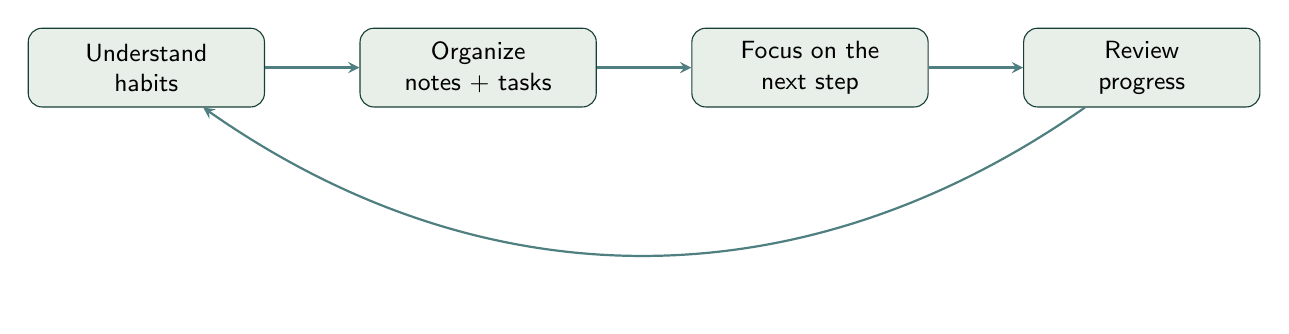
\begin{tikzpicture}[node distance=1.2cm, every node/.style={align=center,font=\small}, box/.style={draw=CognivaForest,fill=CognivaMist,rounded corners=5pt,minimum width=3cm,minimum height=1cm}, arrow/.style={->,>=stealth,draw=CognivaTeal,thick}]
\node[box] (a) {Understand\\habits};\node[box,right=of a] (b) {Organize\\notes + tasks};\node[box,right=of b] (c) {Focus on the\\next step};\node[box,right=of c] (d) {Review\\progress};
\draw[arrow] (a)--(b);\draw[arrow] (b)--(c);\draw[arrow] (c)--(d);\draw[arrow,bend left=35] (d) to (a);
\end{tikzpicture}
\end{center}

\subsection*{Feature naming}
\begin{tabularx}{\textwidth}{>{\bfseries}p{4cm}X}
Notes & Cogniva Notes / AI Summary\\
Tasks & Priority Board / Next Tasks\\
Focus & Adaptive Focus / Focus Session\\
Analytics & Progress / Learning Insights\\
Assessment & Academic Snapshot\\
Assistant & Cogniva Study Assistant
\end{tabularx}

Avoid calling every feature “AI”. Use AI only where a generative or predictive model is actually involved. Fuzzy prioritization can be described as adaptive logic or an explainable priority engine.

\newpage\sectiontitle{08 — Copy examples}
\subsection*{Landing page}
\textbf{Headline:} Make progress easier to see.\\
\textbf{Subheadline:} Cogniva brings your notes, tasks, focus time, and learning patterns into one calm workspace.\\
\textbf{Primary CTA:} Start your workspace\\
\textbf{Secondary CTA:} See how it works

\subsection*{Product microcopy}
\begin{tabularx}{\textwidth}{>{\bfseries}p{4cm}X}
Priority explanation & “This task is high priority because its deadline is near and its difficulty is high.”\\
Focus recommendation & “A 40-minute session gives this task enough room without overloading your focus.”\\
Empty notes & “Your ideas have room here. Add your first note when you’re ready.”\\
Completed session & “Good work. One focused session moved this task forward.”\\
Low confidence insight & “This is an early pattern, not a final conclusion. Keep checking in.”
\end{tabularx}

\subsection*{Accessibility copy rule}
Every important chart, status, or recommendation must have a text explanation. Use descriptive labels, visible focus states, sufficient contrast, and never communicate urgency with color alone.

\newpage\sectiontitle{09 — Brand applications}
\subsection*{Recommended applications}
\begin{itemize}
\item Web application: Ivory canvas, Forest navigation, Teal active states, Sage progress surfaces.
\item Desktop application: App mark on Forest or Ivory; keep the title bar quiet and functional.
\item Social profile: App mark only, centered with generous padding.
\item Academic report: Full lockup on Ivory; use Forest headings and Teal data accents.
\item Presentation: One key idea per slide; use the tagline only on opening or closing slides.
\end{itemize}

\subsection*{Asset checklist}
Before release, maintain these production assets:
\begin{tabularx}{\textwidth}{>{\bfseries}p{4cm}X}
Logo files & SVG primary, SVG monochrome, PNG transparent, favicon, app icon.\\
Color tokens & CSS variables and design-token JSON for Forest, Sage, Teal, Ivory, Ink.\\
Typography & Inter webfont files or hosted font configuration with fallback stack.\\
UI library & Buttons, cards, badges, charts, empty states, focus states, error states.\\
Copy library & Approved headlines, CTA labels, recommendation language, AI disclaimers.
\end{tabularx}

\newpage\sectiontitle{10 — Governance}
\subsection*{Version 1.0 decisions}
This first guideline establishes Cogniva as calm, intelligent, explainable, and progress-oriented. The logo shown in this document is a visual concept direction; production SVG tracing and final typeface licensing should be completed before public launch.

\subsection*{Review checklist}
\begin{itemize}
\item Does the design feel calm before it feels clever?
\item Can the user understand the next action in under five seconds?
\item Is the recommendation explained in plain language?
\item Does the logo remain clear at favicon size and in monochrome?
\item Are claims about AI, prediction, performance, and providers accurate?
\item Does the experience encourage sustainable progress rather than pressure?
\end{itemize}

\vfill\begin{center}\color{CognivaForest}\Large\bfseries Cogniva\\[4pt]\normalsize\color{CognivaTeal} Turn habits into progress.
\end{center}
\end{document}
